\chapter{AFD parte II}
\textbf{Ejemplo: }Del ejemplo de la anterior clase.
%grafico1
\begin{figure}[h!]
\centering
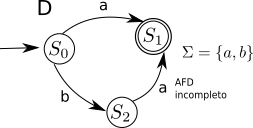
\includegraphics[width=0.4\textwidth]{img_9_1.png}
\caption{AFD incompleto}\label{img_9_1}
\end{figure}


Para que el autómata $D$ se vuelva completo se debe añadir un estado muerto.

%grafico2
\begin{figure}[h!]
\centering
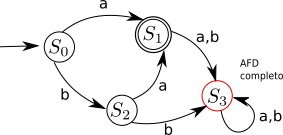
\includegraphics[width=0.4\textwidth]{img_9_2.png}
\caption{AFD completo}\label{img_9_2}
\end{figure}

\textbf{Definición: }Un AFD es conexo si todos sus estaso son accesibles desde el estado inicial.

\textbf{Definición: }En un autómata que no es conexo, se llamará la \textbf{parte conexa} del autómata al conjuto de estados accesibles desde el estado inicial.

\textbf{Ejemplo: }Dibuje un AFD no conexo y determine su parte conexa.
%grafico3
\begin{figure}[h!]
\centering
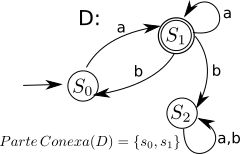
\includegraphics[width=0.4\textwidth]{img_9_3.png}
\caption{Diagrama AFD $D$}\label{img_9_3}
\end{figure}

\textbf{Definición: }Sea un AFD $D=(S,I,\delta,s^*,F)$, llamaremos función de transición extendida a $\widehat{\delta}$ que actúa no solo sobre símbolos sino sobre cadena de símbolos. $\widehat{\delta}$ la definimos recursivamente como sigue:
\begin{enumerate}
\item $\widehat{\delta}(s;\varepsilon)=S \qquad \forall s\in S$
\item (parte recursiva) $\widehat{\delta}(s,au) = \widehat{\delta}(\delta(s,a),u)\qquad a\in \Sigma^* \qquad u\in I^*$

OBS: Notar que $\widehat{\delta}(s,a)=\delta(s,a)$
\begin{align*}
\widehat{\delta}(s,a)&=\widehat{\delta}(s,a.\varepsilon)	\\
				&=\widehat{\delta}(\downlegend{\delta(s,a)}{Estado sgte},\varepsilon) \\
				&=\delta(s,a)
\end{align*}
\end{enumerate}

\textbf{Ejemplo: }Para el AFD $D$

%grafico4
\begin{figure}[h!]
\centering
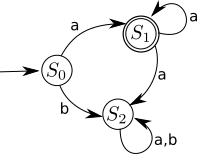
\includegraphics[width=0.3\textwidth]{img_9_4.png}
\caption{Diagrama de Transición de $D$}\label{img_9_4}
\end{figure}
Obtener:
\begin{itemize}
\item $\widehat{\delta}(s_0,a)$
\item $\widehat{\delta}(s_0,ab)$
\item $\widehat{\delta}(s_0,baba)$
\end{itemize}
Usaremos la evaluación rápida.

\textbf{Solución: }
\begin{itemize}
\item $\widehat{\delta}(s_0,a)=\delta(s_0,a)=s_1$

	$s_0\xrightarrow{a} \underline{s_1}$
\item $\widehat{\delta}(s_0,ab)=s_2$

	$s_0\xrightarrow{a}s_1\xrightarrow{b}\underline{s_2}$
\item $\widehat{\delta}(s_0,baba)=s_2$

camino: $s_0\xrightarrow{b}s_2\xrightarrow{a}s_2\xrightarrow{b}s_2\xrightarrow{a}\underline{s_2}$
\end{itemize}
\textbf{Ejemplo: }Sea el AFD $D$, con $\Sigma=\{0,1\}$.

%grafico5
\begin{figure}[h!]
\centering
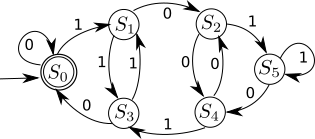
\includegraphics[width=0.4\textwidth]{img_9_5.png}
\caption{Diagrama de Transición de $D$}\label{img_9_5}
\end{figure}

Donde $s^*=s_0$, $F=\{s_0\}\rightarrow\mbox{estado de aceptación}$

Obtener: $\widehat{\delta}(s_0,w)$ para $w=1010$, usando la definición recursiva.
\begin{align*}
\widehat{\delta}(s_0,\downlegend{1}{a}\underbrace{010}_{u})&=\widehat{\delta}(\delta(s_0,1),010)	\\
				&=\widehat{\delta}(s_1,\downlegend{0}{a}\underbrace{10}_{u})	\\
				&=\widehat{\delta}(\delta(s_1,0),10)	\\
				&=\widehat{\delta}(s_2,\downlegend{1}{a}\downlegend{0}{u})	\\
				&=\widehat{\delta}(\delta(s_2,1),0)	\\
				&=\widehat{\delta}(s_5,0)	\\
				&=\delta(s_5,0)	\\
				&= s_4
\end{align*}

$w$ no es aceptada por $D$, para ser aceptada debió acabar en $s_0$.

\textbf{Definición: }El lenguaje reconocido por un autómata $D=(S,I,\delta,s^*,F)$ es el conjunto:
$$L(D)=\{ w\in I^*/\widehat{\delta}(s^*,w)\in F\}$$

Son todas las cadenas aceptadas por el autómata.

\textbf{Ejemplo: }Identifique los elementos del AFD $D$ cuyo lenguaje está dado por el siguiente conjunto:
$$L(D)=\{ w\in I^*/ w \mbox{ tiene un número par de símbolos}\}$$
$$I=\{0,1\}$$

Para el autómata $D=(S,I,\delta,s^*,F)$ se tiene: 
\begin{align*}
I=&\{0,1\}	\\
S=&\{S_{par},S_{impar}\}	\\
F=&\{S_{par}\} \qquad \rightarrow\mbox{Estado de aceptación}	\\
s^*= &S_{par}
\end{align*}
Su tabla de transición será:
\begin{center}
\begin{tabular}{r|cc}
	&\multicolumn{2}{c}{$\delta$}	\\
+	&0		&1	\\ \hline
$(*)\rightarrow S_{par}$	&$S_{impar}$	&$S_{impar}$	\\
$S_{impar}$	&$S_{par}$	&$S_{par}$

\end{tabular}
\end{center}
(*):Tenemos longitud de cadena par + $0$ =$S_{impar}$

Su diagrama de estados:

%grafica6
\begin{figure}[h!]
\centering
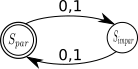
\includegraphics[width=0.2\textwidth]{img_9_6.png}
\caption{Diagrama de Transición de $D$}\label{img_9_6}
\end{figure}

\textbf{Ejemplo: }Identifique los elementos del AFD $D$ que reconoce el lenguaje:
$$L(D)=\{w\in I^*/ w \mbox{ tiene un número}\overbrace{\mbox{ par de 0's}}^{P}\mbox{ y un número} \underbrace{\mbox{impar de 1's}}_{P}\}$$

Dibuje su tabla y diagrama de transición, $I=\{0,1\}$.
\begin{align*}
s^*=&PP	\\
S=&\{\uplegend{P}{(1)}\uplegend{P}{(2)},\downlegend{P}{(3)}\downlegend{I}{(4)},IP,II\}	\\
F=&\{PP\}
\end{align*}
(1):par de 0's; (2):par de 1's; (3):par de 0's; (4):impar de 1's.

Donde:
\begin{itemize}
\item PP: cantidad par de ceros y cantidad par de unos.
\item PI: cantidad par de ceros y cantidad impar de unos.
\item IP: cantidad impar de ceros y cantidad par de unos.
\item II: cantidad impar de ceros y cantidad impar de unos.
\end{itemize}

\begin{center}
\begin{tabular}{c|cc}
	&\multicolumn{2}{c}{$\delta$}\\
+	&0	&1	\\ \hline
$(*)\rightarrow$PP	&IP	&PI	\\
PI	&II	&PP	\\
IP	&PP	&II	\\
II	&PI	&IP	
\end{tabular}
\end{center}
(*): PP le aumentamos $0$ y quedaría cantidad impar de ceros, 1's no varían.

Diagrama:

%grafico7
\begin{figure}[h!]
\centering
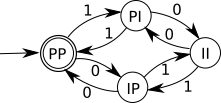
\includegraphics[width=0.4\textwidth]{img_9_7.png}
\caption{Diagrama de Transición de $D$}\label{img_9_7}
\end{figure}

\section{Minimización de un AFD}

\textbf{Definición: }Dos estados $s_1,s_2\in S$ se dirán equivalentes, denotándolos por $s_1\simeq s_2$, si $\forall w\in I^*$:
$$\widehat{\delta}(s_1,w)\in F \Leftrightarrow \widehat{\delta}(s_2,w)\in F$$

Es decir las transiciones que parten de ellos para cada uno de los símbolos del alfabeto llevan al mismo estado $0$ a estados que son equivalentes entre si:

\textbf{Definición: }Un AFD $D$ se llamará autómata mínimo para el lenguaje $L(D)$ si ningún AFD $M$ para $L(M)$ contiene un menor número de estados que $D$.

\section{Algoritmo de Minimización de Estados de un AFD}

\textbf{Objetivo: } Agrupar estados equivalentes para conseguir un AFD equivalente al original.

Pasos:
\begin{enumerate}
\item Vamos a construir una partición $\pi$ de $S$ formada por dos componentes: los estados de aceptación y los que no son.
\item Refinar la partición separando en diferentes componentes a los estados que no son equivalentes.
\item Terminar cuando cada componente de la partición, agrupa estados equivalentes.
\end{enumerate}

\textbf{Ejemplo: }Minimizar el AFD $D$ siguiente(Figura \ref{img_9_8}):

%grafico8
\begin{figure}[h!]
\centering
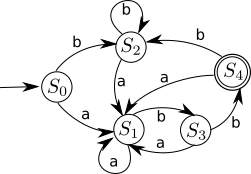
\includegraphics[width=0.4\textwidth]{img_9_8.png}
\caption{Diagrama de Transición de $D$}\label{img_9_8}
\end{figure}

$$\Sigma=\{a,b\} \qquad, s^*=s_0$$

\textbf{Solución: }Tenemos $I=\{a,b\}; S=\{s_0,s_1,s_2,s_3,s_4\}; F=\{s_4\}$.

\begin{enumerate}
\item Construimos $\pi=\{P_1,P_2\}$
\begin{align*}
P_1=&\{s_4\} \\
P_2=&\{s_0,s_1,s_2,s_3\}
\end{align*}
Evaluamos $P_2$ en $I$
\begin{center}
\begin{tabular}{c|cl}
	&\multicolumn{2}{c}{$\delta$}\\
	&a	&b	\\ \hline
$s_0$	&$s_1\in P_2$	&$s_2\in P_2$	\\
$s_1$	&$s_1\in P_2$	&$s_3\in P_2$	\\
$s_2$	&$s_1\in P_2$	&$s_2\in P_2$	\\
$s_3$	&$s_1\in P_2$	&$s_4\not\in P_2,\in P_1\rightarrow (*)$
\end{tabular}
\end{center}
(*): No es estado equivalente. $s_3$ no es equivalente a los estados $s_0,s_1,s_2$.

\item Refinamos la partición $\pi=\{P_1,P_2,P_3\}$
$$P_1=\{s_4\},\qquad P_2=\{3\},\qquad P_3=\{s_0,s_1,s_2\}$$
Analizamos $P_3$ en $I$.
\begin{center}
$\begin{array}{c|cl}
	&a	&b	\\ \hline
s_0	&s_1\in P_3	&s_2\in P_3	\\
s_1	&s_1\in P_3	&s_3\in P_2\rightarrow (1)	\\
s_2	&s_1\in P_3	&s_2\in P_3

\end{array}$
\end{center}
(1): No es estado equivalente. $s_1\not\simeq s_0,s_2$.
\item Refinamos la partición $\pi=\{P_1,P_2,P_3,P_4\}$.
$$P_1=\{s_4\},\qquad P_2=\{s_3\},\qquad P_3=\{s_1\},\qquad P_4=\{s_0,s_2\}$$
Analizamos $P_4$ en $I$.
\begin{center}
$\begin{array}{c|cc}
	&a	&b \\ \hline
s_0	&s_1\in P_3	&s_2\in P_4	\\
s_2	&\underbrace{s_1\in P_3}_{Equivalencia}	&\underbrace{s_2\in P_4}_{Equivalencia}
\end{array}$
\end{center}
Ya no es posible hacer mas refinamientos.

%grafico9
\begin{figure}[t!]
\centering
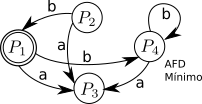
\includegraphics[width=0.4\textwidth]{img_9_9.png}
\caption{Diagrama de Transición del AFD $D$ mínimo}\label{img_9_9}
\end{figure}
\end{enumerate}
